				\documentclass[10pt,a4paper]{article}
				\usepackage[english]{babel}
				\usepackage[utf8]{inputenc}
				\usepackage{fancyhdr}
				\usepackage{hyperref}
				\usepackage{graphicx}
				\usepackage{subcaption}
				\usepackage{caption}
				\usepackage{cite}
				\usepackage{booktabs}
				\usepackage{wrapfig}
				\usepackage{float}
				\usepackage{amsmath}
				\usepackage{xcolor}
				\usepackage{listings}
				\lstset{
					basicstyle=\ttfamily,
					columns=fullflexible,
					frame=single,
					breaklines=true,
					%postbreak=\mbox{\textcolor{red}{$\hookrightarrow$}\space},
				}
				
				\restylefloat{table}
			
				\pagestyle{fancy}
				\fancyhf{}
				\rhead{\today}
				\lhead{Assignment 05}
				\rfoot{Page \thepage}
			
				\begin{document}
				\begin{titlepage}
				\centering
			
					{\scshape\LARGE Scientific Experimentation and Evaluation\par}
			
					{\scshape\Large Assignment: 05\par}
			
					\vfill
			
					\vfill
					{\Large\itshape Anees Khan (9030423)
						\\Debaraj Barua (9030412)\\
						Md Zahiduzzaman (9030432)
						\par}
					\vfill
			
					{\large 14-June-2018\par}
				\end{titlepage}
				\tableofcontents
				\listoffigures	
				\listoftables
				\newpage
				\section{Relevant Aspects of Experiment}
				\subsection{Apparatus}
					\subsubsection{Hardware}
						\begin{itemize}
							\item KUKA youBot arm.
							\item Objects of three different sizes and weights, with ArUco markers attached to the top.
							\item Camera (Microsoft LifeCam).
							\item Two computers, one to run the robot and other for data gathering from the camera.
							\item A fixed container or marker on the table to ensure that the initial object position is kept constant.
						\end{itemize}
					\subsubsection{Software and Libraries used}
						\begin{itemize}
							\item KUKA youBot drivers.
							\item Control scripts for the arm to pick and move the objects in one of the three predefined placing poses.
							\item Marker pose subscribed script, to gather pose of the object.
							\item \textbf{LibreOffice Calc} for data management.
							\item \textbf{Python} for data visualization and calculations
							\item Python libraries:
							\begin{itemize}
								\item pandas
								\item numpy
								\item matplotlib
								\item seaborn
								\item scipy.stats
							\end{itemize}
							\end{itemize}		
											
				\subsection{Procedure}	
					\begin{itemize}
						\item First we run the script to get the arm in the pre-grasp position.
						\item We then place the object in the container, keeping the marker's orientation constant throughout the experiment.\\
						\item We then run the script to move the arm in one of the three pre-defined positions; and repeat this twenty times for each weight and pose combination. Thus, giving us 180 readings of pose coming from three different objects in three different orientations.
						\item Once the object is placed and the arm moves back to a stationary position, we run the subscriber script to collect pose readings of 50 frames from the camera. This is repeated after each motion.
					\end{itemize}
				\subsection{Expected Problems and Performance}
					\begin{itemize}
						\item The picking position of the arm might differ from the ground truth, because of vibrations, motion in the table and a variety of other physical conditions.
						\item The placement of the object in the container might not always be aligned properly.
						\item The marker on top of the object might move during movement and thus will lead to improper pose data.
						\item After placing the object, the gripper might touch it while moving away, which will introduce distortions in data.
						\item The light might not always be uniform, which might also cause some distortions in observation.						
					\end{itemize}
					
				\section{Observations and Data}
					 \subsection{Visualization}
						 \subsubsection{Data Visualization}
						\begin{itemize}
							\item The raw data with fifty reading for each run has been filtered and saved as an average. This data is used for further visualization. 
							\item The first visualization shows the pose distribution of large, medium and small objects in three directions including the initial and expected pose. 
							\item The upper right hand corner is the left run plot and the lower left hand corner is right run plot.
							\begin{figure}[h]
								\centering
								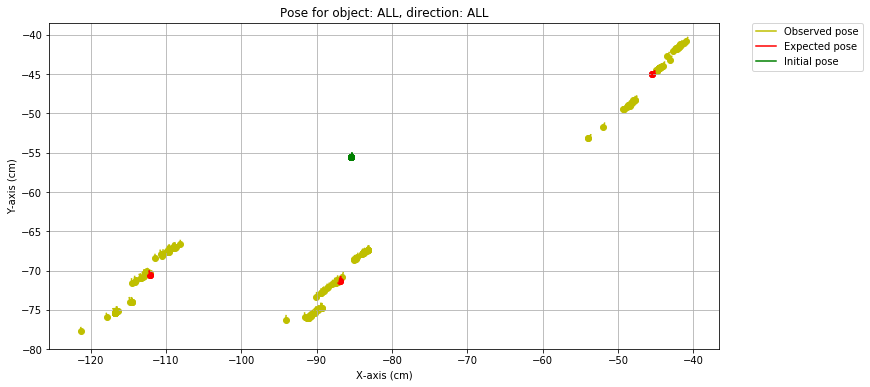
\includegraphics[width=1.0\linewidth]{img/pose_all_all.png}
								\caption{poses for all objects in straight, left and right direction}
								\label{fig:poses for all objects in straight, left and right direction}
							\end{figure}
					\end{itemize}			
	    				 \subsubsection{Outlier Detection and Removal}
		    				 We filtered the noisy raw data by removing all records with x, y or theta value outside the range of $\mu_x \pm 2\sigma_x$, $\mu_y \pm 2\sigma_y$, $\mu_\theta \pm 2\sigma_\theta$ respectively. We used the filtered raw data to calculate mean for each experimental trial. Total number of outlier is 495 and outlier per experimental run is 2.75
						 \subsubsection{Pose Visualization}
							\begin{itemize}
								\item The first section shows the pose plots of small, medium and large objects in straight path. 
								\item It shows the initial pose, the expected(ground truth) and observed pose(twenty points).  
								\item The same process is repeated for left followed by right run.
								
								\begin{figure}[H]
									\begin{subfigure}{0.5\textwidth}
										\centering
										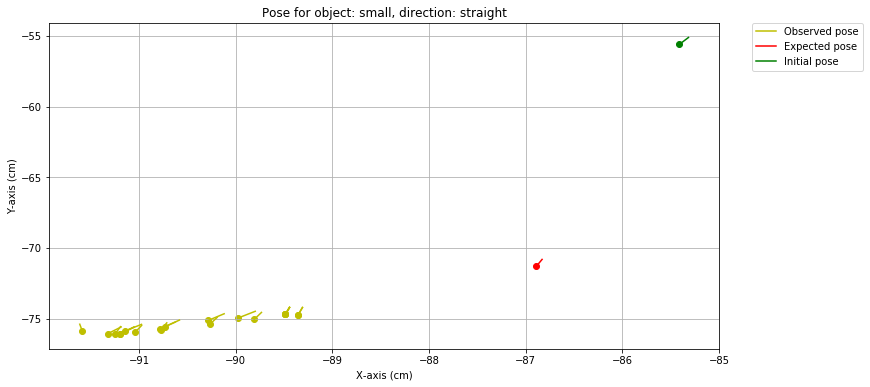
\includegraphics[width=0.8\linewidth]{img/pose_small_straight.png}
										\caption{object: small, direction: straight}
										\label{fig:object: small, direction: straight}
									\end{subfigure}%
									\begin{subfigure}{0.5\textwidth}
										\centering
										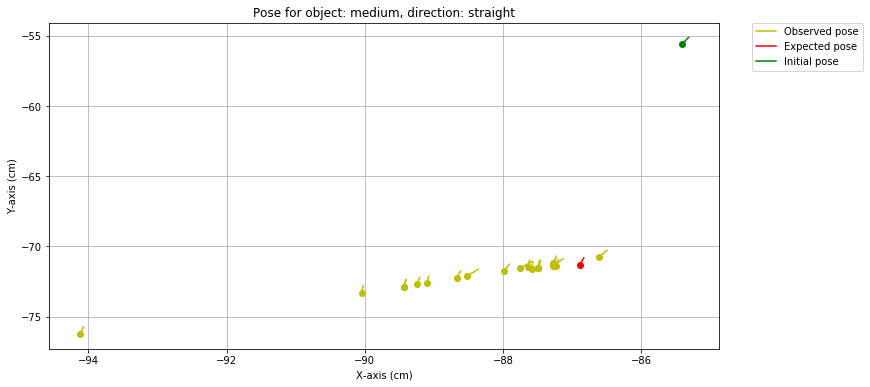
\includegraphics[width=0.8\linewidth]{img/pose_medium_straight.png}
										\caption{object: medium, direction: straight}
										\label{fig:object: medium, direction: straight}
									\end{subfigure}
									
									\begin{subfigure}{0.5\textwidth}
										\centering
										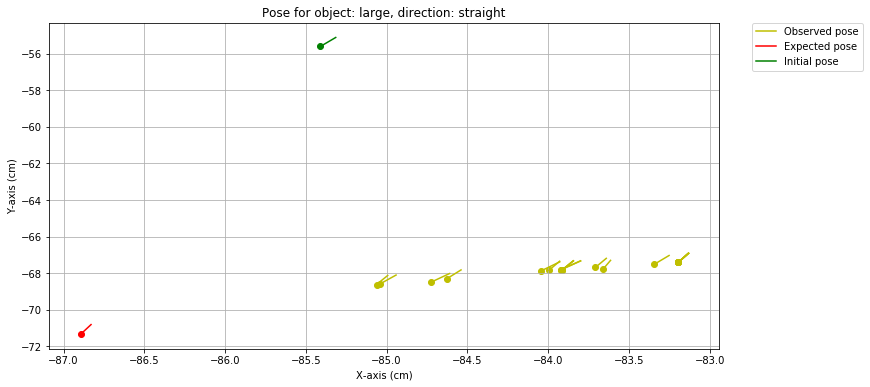
\includegraphics[width=0.8\linewidth]{img/pose_large_straight.png}
										\caption{object: large, direction: straight}
										\label{fig:object: large, direction: straight}
									\end{subfigure}%
									\begin{subfigure}{0.5\textwidth}
										\centering
										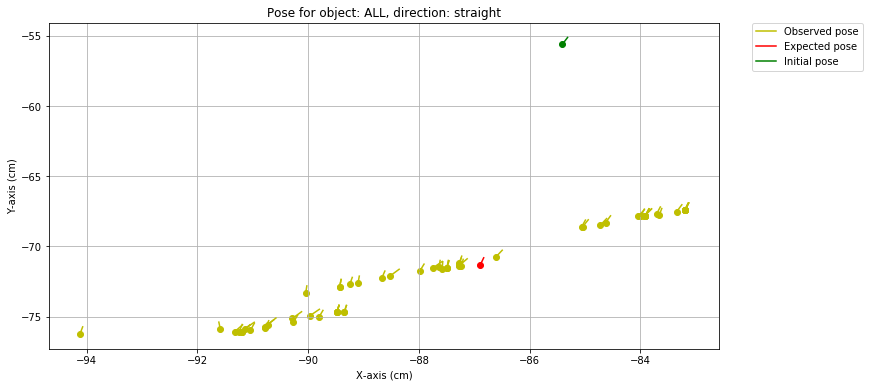
\includegraphics[width=0.8\linewidth]{img/pose_all_straight.png}
										\caption{object: all, direction: straight}
										\label{fig:object: all, direction: straight}
									\end{subfigure}
									
									\caption{pose in straight direction}
									\label{fig:pose in straight direction}
								\end{figure}
								
								\begin{figure}[H]
									\begin{subfigure}{0.5\textwidth}
										\centering
										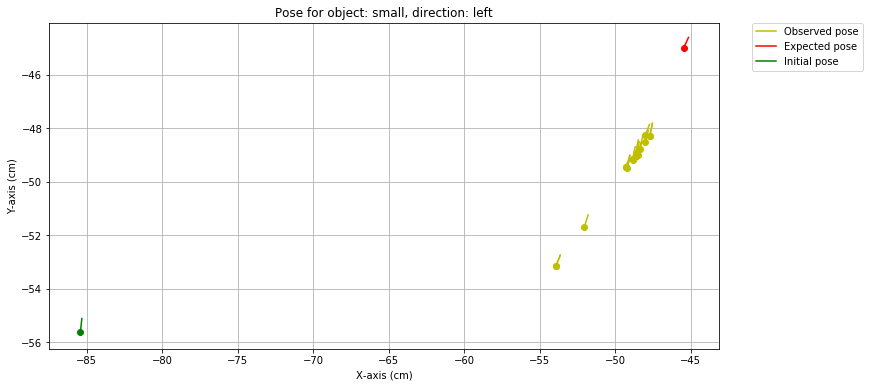
\includegraphics[width=0.8\linewidth]{img/pose_small_left.png}
										\caption{object: small, direction: left}
										\label{fig:object: small, direction: left}
									\end{subfigure}%
									\begin{subfigure}{0.5\textwidth}
										\centering
										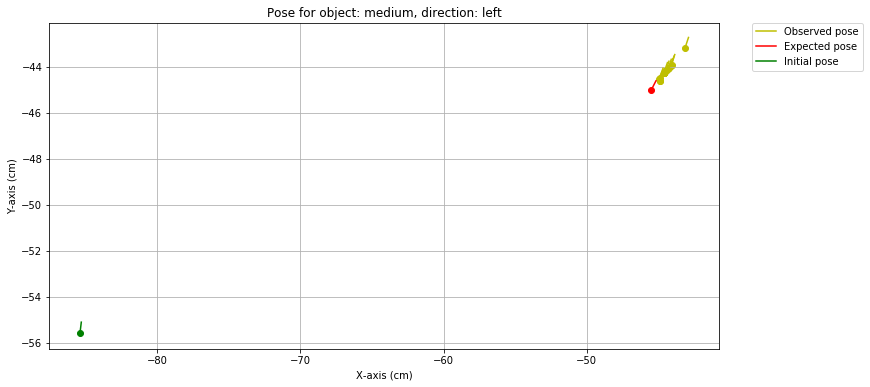
\includegraphics[width=0.8\linewidth]{img/pose_medium_left.png}
										\caption{object: medium, direction: left}
										\label{fig:object: medium, direction: left}
									\end{subfigure}
									
									\begin{subfigure}{0.5\textwidth}
										\centering
										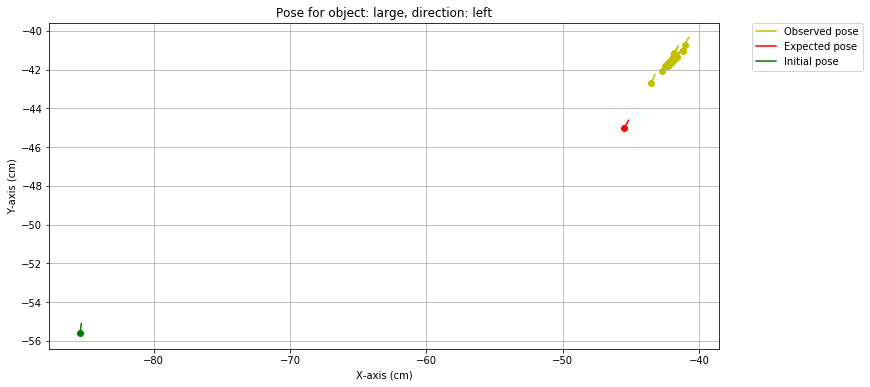
\includegraphics[width=0.8\linewidth]{img/pose_large_left.png}
										\caption{object: large, direction: left}
										\label{fig:object: large, direction: left}
									\end{subfigure}%
									\begin{subfigure}{0.5\textwidth}
										\centering
										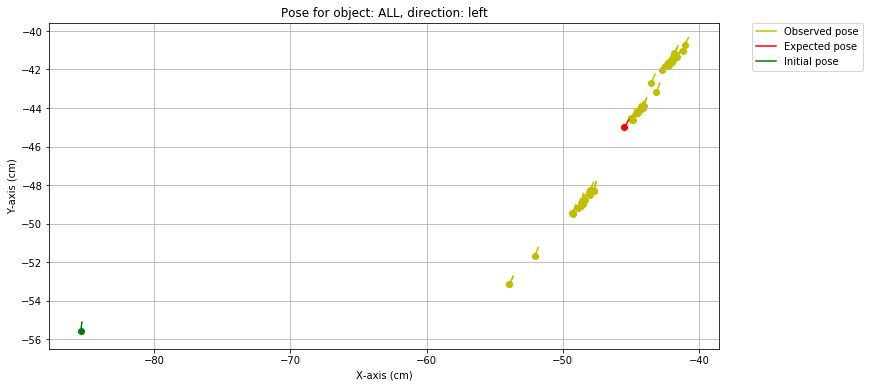
\includegraphics[width=0.8\linewidth]{img/pose_all_left.png}
										\caption{object: all, direction: left}
										\label{fig:object: all, direction: left}
									\end{subfigure}
									
									\caption{pose in left direction}
									\label{fig:pose in left direction}
								\end{figure}
								
								\begin{figure}[H]
									\begin{subfigure}{0.5\textwidth}
										\centering
										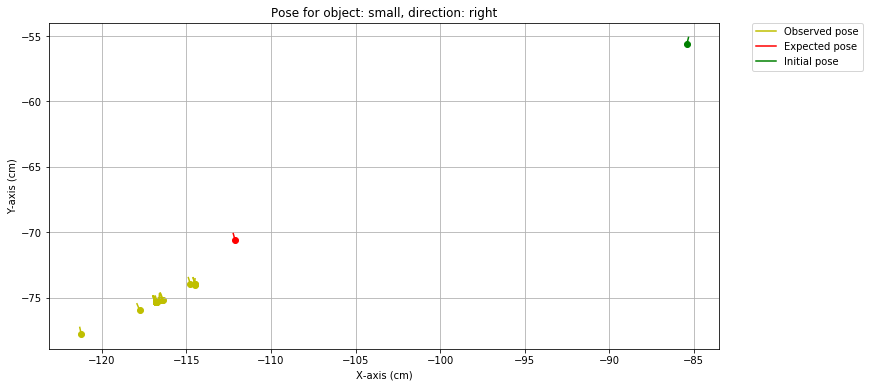
\includegraphics[width=0.8\linewidth]{img/pose_small_right.png}
										\caption{object: small, direction: right}
										\label{fig:object: small, direction: right}
									\end{subfigure}%
									\begin{subfigure}{0.5\textwidth}
										\centering
										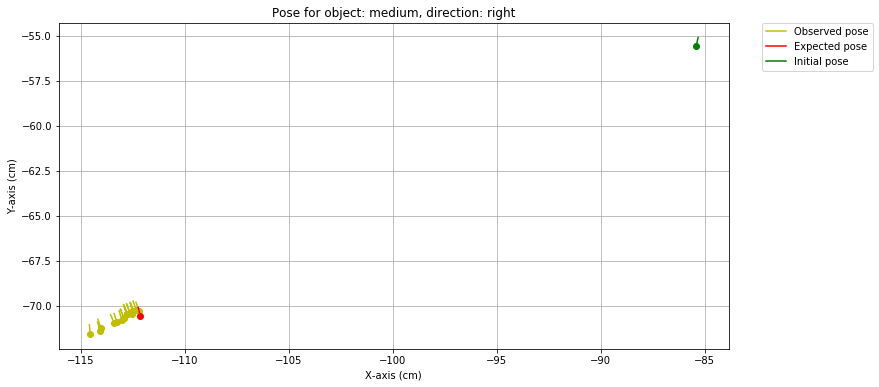
\includegraphics[width=0.8\linewidth]{img/pose_medium_right.png}
										\caption{object: medium, direction: right}
										\label{fig:object: medium, direction: right}
									\end{subfigure}
									
									\begin{subfigure}{0.5\textwidth}
										\centering
										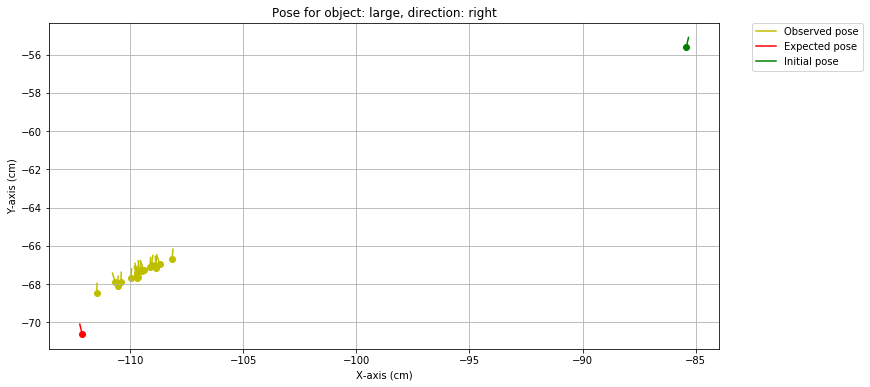
\includegraphics[width=0.8\linewidth]{img/pose_large_right.png}
										\caption{object: large, direction: right}
										\label{fig:object: large, direction: right}
									\end{subfigure}%
									\begin{subfigure}{0.5\textwidth}
										\centering
										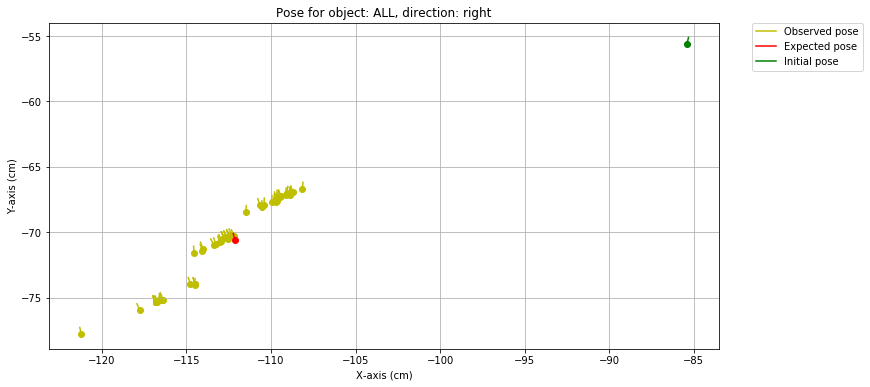
\includegraphics[width=0.8\linewidth]{img/pose_all_right.png}
										\caption{object: all, direction: right}
										\label{fig:object: all, direction: right}
									\end{subfigure}
									
									\caption{pose in right direction}
									\label{fig:pose in right direction}
								\end{figure}

							\end{itemize}	
					\subsubsection{Numerical Results}
							\begin{itemize}
							\item By taking mean of all the all the points for straight, left and right gave us the following numbers. 
							\item Straight: \\
									X-axis: -87.54 \\
									Y-axis: -71.77 \\
									Angle: 1.42	
							\item Left:\\
									X-axis: -45.27\\
									Y-axis: -45.10 \\
									Angle: 0.98
							\item Right:\\
									X-axis: -113.04\\
									Y-axis: -71.08 \\
									Angle: 1.76

							\end{itemize}		
					
%				\section{\textcolor{blue}{Results}}
%				\subsection{Final Position \& Accuracy }
%				  \textcolor{red}{Display in a tabular format}
%				\subsection{Compare Data with Gaussian}
				\end{document}
